\subsection{Stage 5b --- NN-Driven MEAM Parameter Optimization}
\label{sec:nnip}

Stage~5b is the part that closes the loop. It refits the cross-interaction
terms of the merged Stage~4 library so the potential reproduces the
LAMMPS-evaluated elastic targets. Doing this directly would mean a LAMMPS run
inside every optimizer step, which is far too slow. Instead a neural network
learns the forward map from MEAM parameters to elastic constants, and the
optimizer works against that cheap differentiable surrogate. The loop has four
parts.

\paragraph{Sample.}
Starting from the Stage~4 baseline $\mathbf{p}_0$, the stage draws $N$
perturbed parameter vectors
$\mathbf{p}_k = \mathbf{p}_0 \cdot (1+\boldsymbol{\eta}_k)$ with
$\eta_k\sim\mathcal{U}(-0.1,0.1)$ applied to each binary
$(\texttt{Ec},\texttt{re},\texttt{alpha})$ triple. Every sampled vector is
written into a MEAM file and run through LAMMPS over a representative set of
alloys to obtain $(C_{11},C_{12})_k$ per composition. The representative set
is a $k$-means-medoid reduction of the full Stage~2 database, which keeps the
sampling cost down while still spanning the composition space. A sample whose
majority of compositions fail a $C_{11}>30$\,GPa check is thrown out before it
can pollute the training set.

\paragraph{Train a surrogate.}
A feed-forward network is fit on the surviving samples, mapping the parameter
vector to the per-composition $(C_{11},C_{12})$ under a Huber loss
\citep{tensorflow2015}. Predicting the stiffness constants rather than $\nu$,
and using a robust loss, are the two lessons carried over from the composition
surrogate of Section~\ref{sec:comp_nn}. The surrogate Huber loss falls from
$1.0$ to about $0.16$ over $10^4$ optimizer steps
(Figure~\ref{fig:nnip_loss}).

\paragraph{Inverse optimization.}
With the surrogate $f_\theta$ trained, the refit parameters are found by
$\hat{\mathbf{p}} = \arg\min_{\mathbf{p}}\,\lVert f_\theta(\mathbf{p}) -
\mathbf{y}^\star\rVert$, again under the Huber loss, with L-BFGS
\citep{liu1989lbfgs} descending on the normalised parameter vector. The search
is clipped to $\pm2.5\sigma$ around the training mean so the optimizer cannot
wander outside the region where the surrogate is trustworthy.

\paragraph{Re-evaluate and repeat.}
The refit vector $\hat{\mathbf{p}}$ is run back through LAMMPS, the new samples
are appended to the training set, and the surrogate is retrained. Every stage
writes its output to a deterministic location and checkpoints atomically, so a
run that is interrupted resumes from where it stopped rather than restarting.
An active-learning variant focuses the next sampling round on the parameter
regions the surrogate is least sure about.

\paragraph{Results.}
The refit potential was validated on 30 held-out alloys by re-running them in
LAMMPS and comparing against the MD targets. The outcome is honest but mixed
(Figure~\ref{fig:nnip_errors}). Of the 30, only 11 pass the Born--Cauchy
stability filter; the other 19 come out mechanically unstable
($C_{11}<C_{12}$). Among the 11 stable alloys the median error is $23\,\%$ on
$E$ and $26\,\%$ on $\nu$, and 4 fall within the $20\,\%$ tolerance on both.
The instability is concentrated, as expected, in the non-aluminium chemistries
where the Stage~2 sampling and the DFT reference are both thinnest. Inside the
aluminium-rich region the refit holds up well, which the external validation
of Section~\ref{sec:validation} quantifies. The gap on the unstable 19 is the
clearest signal of where the method needs more work, and it sets the agenda in
Section~\ref{sec:future}.

\begin{figure}[h]
	\centering
	\begin{minipage}[t]{0.48\textwidth}
		\centering
		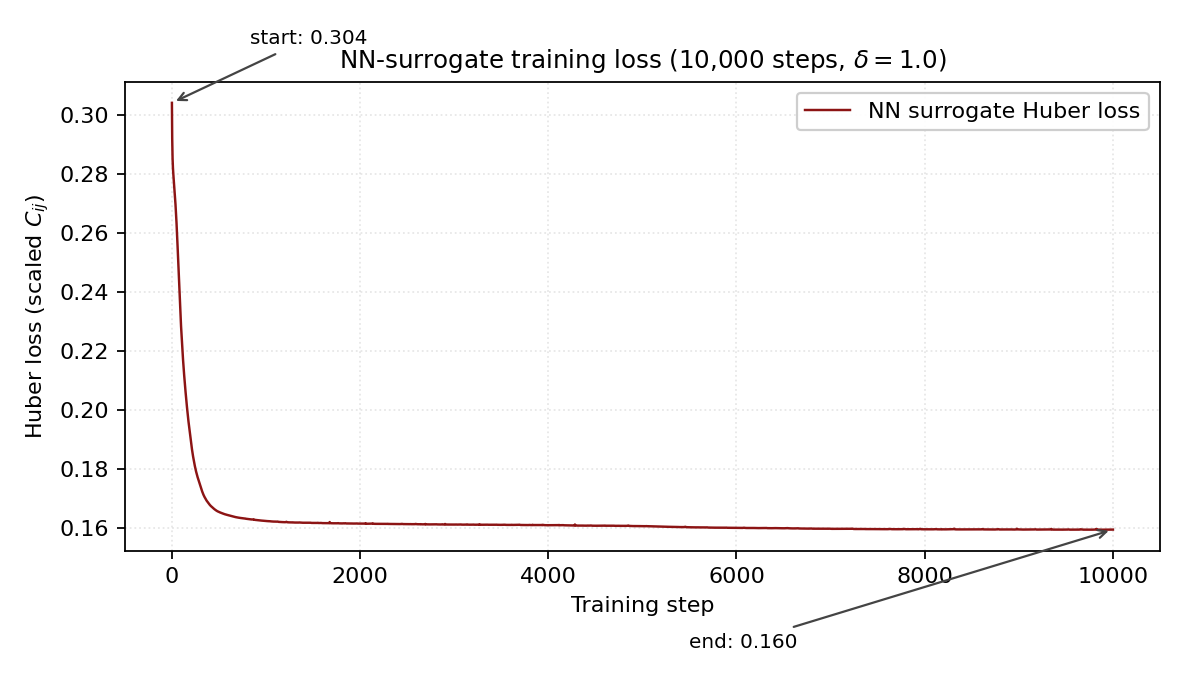
\includegraphics[width=\textwidth]{figures/nnip_training_loss.png}
		\caption{Surrogate Huber loss over $10^4$ optimizer steps, falling from
		$1.0$ to about $0.16$.}
		\label{fig:nnip_loss}
	\end{minipage}
	\hfill
	\begin{minipage}[t]{0.48\textwidth}
		\centering
		
\includegraphics[width=\textwidth]{figures/nnip_verification_errors.png}
		\caption{Verification error on the 30 held-out alloys, with a separate
		bar for the runs rejected as mechanically unstable.}
		\label{fig:nnip_errors}
	\end{minipage}
\end{figure}

\begin{figure}[h]
	\centering
	
\includegraphics[width=0.7\textwidth]{figures/nnip_stage_timings.png}
	\caption{Per-stage wall-clock time for one full Stage~5b cycle (log scale).
	The LAMMPS sampling dominates; the surrogate training and inverse
	optimization are comparatively cheap, which is exactly why the surrogate is
	worth building.}
	\label{fig:nnip_timings}
\end{figure}
